\chapter{Ist-Analyse}
\label{chap:ist-analyse}

Dieses Kapitel dient der Beschreibung existierender Systeme.
Es soll ihre Eigenschaften und Probleme aufzeigen.
Diese werden zuerst theoretisch betrachtet und
dann an Systemen in der Praxis demonstriert.

% dieses kap dient .. und damit soll .. aufbau

\section{Eigenschaften der existierenden Systeme}

\subsection{Struktur}
\label{sec:ist-analyse:struktur}

Wie in der \cref{fig:ist-aufbau-tradition} leicht zu erkennen ist,
sind traditionellen \ac{CI}-Systeme Client-Server Systeme.

\begin{figure}[ht]
  \centering
  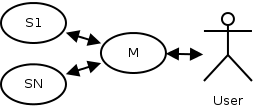
\includegraphics[height=1in]{imageinput/ist-aufbau-tradition.png}
  \caption{Logischer Aufbau eines CI System}
  \label{fig:ist-aufbau-tradition}
\end{figure}

Der sogenannte Master (M) ist der Server und verwaltet alle Daten.
Die Slaves (S1 bis SN) sind die Clients und verrichten die eigentliche Arbeit.
Sie sammeln Daten und liefern diese einschließlich der Resultate beim Master ab.

Benutzer interagieren ausschließlich mit dem Master.

\subsection{Datensammlung}
Wie bereits in \Cref{sec:base:ci} erwähnt,
führt ein \ac{CI}-System nicht nur Aufträge aus,
sondern sammelt auch Daten für die spätere Weiterverarbeitung.

Die Datensammlung lässt sich dabei grob in zwei Bereiche einteilen:
Zum einen in die Laufzeitdaten und zum anderen in die Artefakte.

Laufzeitdaten fallen bereits w\"ahrend der Ausf\"uhrung an
und beinhalten in der Regel zumindest die textuellen Ausgaben
der ausgef\"uhrten Programme.
Weitere M\"oglichkeiten k\"onnen Resultate von Tests, Echtzeitmitschnitte und Ausführungsstatistiken sein.
Laufzeitdaten werden dem Benutzer in der Regel zeitnah zur Verfügung gestellt.

Artefakte hingegen sind Dateien,
welche erst nach Abschluss eines Schrittes zur Verfügung stehen.
Zu ihnen geh\"oren neben den traditionellen, ausf\"uhrbaren Dateien
auch lauff\"ahige Archive des Gesamtprogramms oder Testergebnisse in Formaten wie z.B. JunitXML \cite{jenkins:junitxml} oder \ac{TAP}.

%XXX: cite tap, junitxml

Diese werden zum Master geschickt, dort aufbewahrt und sp\"ater genutzt.

In der Regel werden ausf\"uhrbare Artefakte zum Download angeboten,
w\"ahrend Testergebnisse nur dargestellt werden.


\section{Probleme existierender Systeme}

Dieses Unterkapitel gibt einen \"Uberblick \"uber die Problemarten existierender Systeme.

\subsection{Datenzugriff}

Beim Datenzugriff sind die existierenden Systeme besonders problematisch.
Es gibt grundsätzlich keinerlei Standardschnittstellen.
Die meisten Systeme verwenden noch nicht einmal eine Datenbank.
Jene, welche doch eine Datenbank verwenden, machen sie nicht zugänglich.

Die Datenhaltung dieser Systeme kann somit grob als geordnete Ablage klassifiziert werden.
Weiterführende Abfragen sind nicht möglich.

\subsection{Erweiterbarkeit}

Die Erweiterbarkeit eines \ac{CI}-Systems wird von zwei Hauptpunkten dominiert.
Dies ist zum einen die Integration in die Benutzeroberfl\"ache
und zum anderen die Möglichkeit mit den Daten zu interagieren
und diese auf neue Weise zu kombinieren.

Die erweiterbaren Systeme stellen normalerweise zumindest eine Schnittstelle
für die graphische Oberfläche zur Verfügung.
Damit ist zumindest das problemlose Anpassen der Benutzeroberfläche gegeben.


Für eigene Analysewerkzeuge kann es jedoch oft notwendig werden,
eine eigene Datenbank, welche vom \ac{CI}-System getrennt ist, zu verwenden.
Einige Anbieter von \ac{CI}-Werkzeugen wünschen dies sogar explizit.


\subsection{Komponentenabhängigkeit}

Wie bereits in \cref{sec:ist-analyse:struktur} erw\"ahnt,
sind \ac{CI}-Systeme in der Regel traditionelle Netzwerksysteme,
die nach dem Client/Server-Prinzip operieren.
Dabei sind die Rollen strikt als Master und Slave eingeteilt.
Das Management wird zentral im Master vorgenommen.
Die Slaves haben dabei keinerlei Autonomie
und folgen strikt den Anweisungen des Masters.

Dadurch nimmt das System zwar keinen Schaden, wenn ein Slave ausfällt,
der Ausfall des Master ist jedoch fatal und kann nicht abgefangen werden.
Dies stellt einen ``Single Point of Failure'' dar.


\section{Beispiele aus der Praxis}

Um Probleme in der Praxis aufzuzeigen,
soll eine Auswahl an Werkzeugen getroffen werden.
Anschließend sollen ihre Eigenschaften und Probleme
näher untersucht werden.


\subsection{Auswahl}

Um die Analyse von Beispielen aus der Praxis zu ermöglichen,
sollen Systeme mit gewissen Rahmenbedingungen ausgew\"ahlt werden.
Wichtigstes Kriterium ist dabei, dass sie \textbf{Open-Source}-Software sind,
oder zumindest öffentlich verfügbar sind.
Sie sollten \textbf{verbreitet} sein, damit ein Überblick
über praxisrelevante Probleme geschaffen werden kann.
Außerdem sollten sie \textit{kostenlos} sein. %,
%XXX> LOL
%\textit{um den finanziellen Ruin eines hilflosen Studenten zu verhindern}.

Ausgewählt wurden die Systeme
\begin{itemize}
  \item \emph{Jenkins/Hudson},
  \item \emph{Buildbot} und
  \item \emph{TravisCI}.
\end{itemize}

Sie alle sind kostenlose Werkzeuge und quelloffen.
Sie decken unterschiedlichste Use-Cases ab.

\subsection{Jenkins/Hudson}

Jenkins und Hudson sind aus der Java-Welt  stammende \ac{CI}-Systeme.
Sie bieten alle Grundfunktionen, um grundlegendes \ac{CI} umzusetzen
und unterst\"utzen auch erweiterte Funktionen,
wie Matrix-Build und nachgelagerte Builds.

Sie stellen ein einfach zu bedienendes Nutzerinterface zur Verfügung,
Konfiguration findet jedoch nur im Rahmen dieses Interfaces statt.

Erweiterte Parametrisierung ist nicht m\"oglich.
Entwicklungszweige sind dem System unbekannt.
M\"ochte man mehr als einen Entwicklungszweig dem Testprozess unterziehen,
so m\"ussen weitere Jobs angelegt werden.

Zugriff auf die Daten kann nur mittels der internen \ac{API} oder
einer nicht dokumentierten \ac{REST} \ac{API} genommen werden.

Damit war es nicht m\"oglich, in annehmbarer Zeit festzustellen,
inwieweit sich die bereits vorgestellten Usecases umsetzen lassen.
Das System verwendet augenscheinlich kein \ac{DBMS}.
Datenabfragen und Aggregationen m\"ussen
somit von Hand ausformuliert werden.

Das Konzept der Build-Artefakte wird unterst\"utzt und
aktiv f\"ur Funktionen wie nachgelagerte Builds verwendet.

Es gibt einige einfach gestrickte Plugins mit dem Zweck die Testresultate anzuzeigen.
Jedoch wird auf weitergehende Analysen dieser Resultate g\"anzlich verzichtet
und mehr als ein Histogramm gibt es nicht.


\subsection{BuildBot}


BuildBot \cite{buildbot:website} positioniert sich als eine Art Meta-Build-Server.
Er bietet keine normale Benutzerschnittstelle zur Konfiguration,
sondern wird mittels Komposition von Metadaten und Komponenten konfiguriert.

Die Konfiguration des Servers stellt dabei ein Python-Script dar,
welches die gewünschten Jobs zusammenstellt und den Server konfiguriert.
Matrix-Builds werden nicht unterst\"utzt,
k\"onnen aber in Teilen durch die Verwendung von Schleifen im Script simuliert werden.
Es ist möglich Build-Jobs mit minimalen Parametern in Form von Strings zu \"ubergeben,
dabei kann man auch den Entwicklungszweig mit angeben.

Builbot unterst\"utzt das Sammeln von Daten in sogenannten Logdateien.
Diese sind intern und extern leicht auffindbar.
Es gibt sogar schon Werkzeuge, welche diese zu erweiterten Vergleichen von Testresultaten nutzen.

%XXX referenzen
%XXX: C
Einige wurden dabei besonders genau betrachtet.
Das erste ist der PYPY-BuildBot \cite{pypy:overview}, welcher eine hilfreiche Gesamtübersicht der Testergebnisse und ihrer Fehler darstellt.
Dabei werden nur die letzten vier Builds betrachtet.
Das zweite ist das Script namens \verb|compare_last_builds.py|
aus dem PYPY Projekt \cite{pypy:diffscript} ,
welches die Unterschiede in den Testresultaten zwischen zwei Builds hervorhebt.
Sie werden sp\"ater als Ideenlieferant dienen.

Bedauerlich ist, dass die Entwickler von BuildBot es nicht als Aufgabe ihres Systems sehen
sich mit Testergebnissen zu befassen.
Sie empfehlen die Integration externer Komponenten \cite{buildbot:irc}.

\subsection{TravisCI}


%XXX refs
TravisCI \cite{travisci:website} ist wesentlich anders positioniert als die beiden vorhergehenden Systeme.
Es stellt Zusammenarbeit in den Vordergrund und der Open-Source-Community werden gehostete Server
kostenfrei zur Verf\"ugung gestellt.
Diese behandeln die Integration von Projekten,
welche auf der beliebten Code-Hosting Seite GitHub verwaltet werden.

% ref yaml % acronym yaml
Die Konfiguration ist dabei zweigeteilt,
eine Datei im \ac{YAML} Format \cite{yaml:website} legt dabei Build-Achsen und Schritte fest.
Diese Datei befindet sich in der Versionskontrolle beim Projekt
(was die Konfiguration sehr flexibel gestaltet).

Ist ein Projekt erst einmal im System registriert,
so wird es regelmäßig bei Änderungen integriert.

Besonders hilfreich ist, dass TravisCI auch den Fall behandelt,
wenn ein anderer Benutzer der Code-Hosting Seite Github \"Anderungen anmeldet
\cite{github:pullreq} (sog. Pull-Request).
Die testet es und f\"ugt anschließend das Resultat der \"Anderungsanmeldung hinzu.

Dies \"andert leider nichts daran, dass TravisCI keine externe API zur Verfügung stellt.
Es ist ein geschlossenes System. Außerdem hat es kein Konzept f\"ur Datensammlung/Artefakte
und auch Testresultate werden nicht betrachtet.
Es ist nicht portabel und scheinbar f\"ur den Betrieb nur
auf den zur Verfügung gestellten Servern vorgesehen.


\section{Zusammenfassung}

Dieses Kapitel hat die Probleme der \ac{CI}-Systeme n\"aher gezeigt.
Wir haben gesehen, dass Datenzugriff und Erweiterungen f\"ur Analyse
schwer oder gar nicht zu erreichen sind.
Außerdem sind die Systeme nach einigen Fehlerklassen nicht direkt wiederherstellbar.
Im folgenden Verlauf der Arbeit soll der Grundstein f\"ur ein \ac{CI}-System gelegt werden,
welches Datenzugriff und Datenanalyse vereinfacht.
Zus\"atzlich soll es eine bessere Fehlertoleranz aufweisen.


